%& --shell-escape --enable-write18 
\documentclass[english]{iambook}
\usepackage[utf8]{inputenc}

\usepackage{amsmath}

\newcommand{\beq}{\begin{eqnarray*}}
\newcommand{\eeq}{\end{eqnarray*}}
\newcommand{\beqn}[1]{\begin{eqnarray}\label{#1}}
\newcommand{\eeqn}{\end{eqnarray}}
\newcommand{\missing}[1]{{\bf missing:}{#1}}
\newcommand{\comment}[1]{{\bf comment:}{#1}}
\newcommand{\nz}{{\if mm {\rm I}\mkern -3mu{\rm N}\else \leavevmode
\hbox{I}\kern -.17em \hbox{N} \fi}}
\newcommand{\calP}{{\cal P}}
\newcommand{\calQ}{{\cal Q}}
\newcommand{\calR}{{\cal R}}
\newcommand{\calS}{{\cal S}}
% \renewcommand{\matrixQ}{{\bf Q}}
\newcommand{\id}{\hspace*{0.2cm} {\if mm {\rm I}\mkern - 11.8mu{\rm 1}\else \leavevmode
\hbox{I}\kern -.17em \hbox{1} \fi}\hspace*{1mm}_\nu \hspace*{0.1cm} }

\newcommand{\vphi}{\mbox{\boldmath{$\phi$}}}
\newcommand{\vc}{\mbox{\boldmath{$c$}}}

\usepackage{subfigure}
\usepackage{graphicx}
\usepackage{tikz}
% \usepackage{tikz-pic}
\usepackage{pgfplots}
\bibliographystyle{plain}

\title{Basics of diffuse interface modeling}
\author{}
\date{}

\begin{document}
\frontmatter
\maketitle
\mainmatter
\chapter{Phase-field modeling}
\section{Introduction}
In materials science and in general a number of physical phenomena
involve motion of boundaries between entities which are homogeneous 
with respect to certain physical properties. These problems fall in 
the realm of what are known as free-boundary or moving 
boundary problems. Examples of such phenomena are solidification, 
precipitation, phase-separation, order-disorder transitions etc.
A notable feature of such problems, involves, mass, heat or momentum 
transfer across \textit{interfaces} which are the boundaries between 
physically homogeneous media (\textit{phases}). Classically, such 
moving boundary problems were modeled using \textit{sharp-interface
methods} where the nodes which discretely represent the interface, 
are explicitly tracked and the appropriate boundary conditions at
the interface are imposed at these boundary nodes, an example being 
the \textit{boundary integral model}. This is however, 
time-consuming and memory intensive when one is intending to numerically
compute using the sharp-interface descriptions of these free-boundary 
problems for large domain computations. In addition, the models are
restrictive/limited in nature as complex geometric evolution involving
multiple curvatures and catastrophic phase evolution are outside the
scope of such models.

A second approach which enables a more elegant treatment of the 
problem are \textit{diffuse-interface models}. Here, the dis-continuity 
in a physical property/quantity across the interface is allowed
to vary over a finite width. The temporal evolution of any phase transformation
is then implicitly tracked by following the evolution of this spatially
continuous field as function of time. The boundary conditions are self-consistently
accounted for in this description and the actual sharp-interface interface
problem is retrieved when the length scale of the diffuse-interface region 
is much smaller compared to the microscopic length scale of the morphological 
feature one is modeling.

The parameter for distinguishing between the phases can be chosen 
among the various extensive variables distinguishing the phases.
Generally, the relevant parameter/s are the ones which are the more
sensitive to the given processing conditions. So for example, for 
case of a pure material solidification, under constant pressure
with equal molar volumes of the phases, the parameter could be 
either the order in the solid/liquid, the internal energy etc.
This parameter which differentiates between the phases is termed
as an \textit{order parameter}. Another example for an 
order parameter is the \textit{composition}.

Another perspective for diffuse-interface models, is to
perceive order-parameters as \textit{indicator-functions}
in which an arbitrary set of spatially continuously varying
functions are used to describe multiple-phases in the system.
This set of parameters is then utilized to describe the variation of
the intensive-extensive variables in the system through the
use of implicit/explicit functions of the order parameter/s.
This is the more elaborately used methodology as is usually
termed the \textit{Phase-field approach}.

It is important to note that, atomistically interfaces
have finite thickness(over some angstroms). So, while this
could be a physical motivation for phase-field/diffuse-interface
formulations, the choice of the difference interface thickness
in the mathematical model has no bearing on the physically 
realistic value. This is because in the model, 
the interface width is a physical construct utilized to elegantly
reproduce the sharp-interface free-boundary problem. Since, 
the physical interface thickness is not present in the 
sharp-interface free-boundary problem, therefore it makes 
the reproduction in the phase-field/diffuse-interface model
unnecessary. The choice of the length-scale of the diffuse
interface is chosen as per the morphological length scale
one is modeling. In the following sections, we will be 
presenting an overview of two models; one based on the 
choice of order-parameter as the composition (\textit{Cahn-Hilliard}), and the 
other where the order parameter is non-conserved(\textit{Allen-Cahn}). Essentially, 
the evolution equations which deterministically describe
the evolution of the order-parameter functions ensure that
the energy of the system is minimized. However, the two 
following descriptions, result in different evolution equations.

\section{Cahn-Hilliard equation}
Consider the diffusion equation for a single phase
material with two components,
\begin{align}
 \dfrac{\partial c}{\partial t} &= -\nabla\cdot\mathbf{J} = \nabla\cdot\left(M\nabla\mu\right) = D\dfrac{\partial ^{2}c}{\partial x^{2}}
\end{align}

which is a statement of mass-conservation, with the flux being written solely
proportional to the gradient of the diffusion potential $\mu=\mu_A- \mu_B$ and $M$ being the mobility
of the atoms, $M=D/\dfrac{\partial \mu}{\partial c}$ . 
At equilibrium, $\dfrac{\partial c}{\partial t}=0$, the concentration 
profile can be solved for, to be linear between the values at
the boundaries.

Now, consider a system of two phases in equilibrium with
compositions $c^{\alpha}$ and $c^{\beta}$. Clearly, if we 
were to write a single thermodynamically consistent equation, 
for the entire system, $\dfrac{\partial c}{\partial t} 
= D\dfrac{\partial^{2}c}{\partial x^{2}}$
cannot remain valid, since this would imply, that in the 
event of no-flux (Neumann) boundary conditions (a closed system) 
a uniform composition field would be the equilibrium state of
the system that clearly violates the thermodynamically derived
equilibrium state of the system (equal chemical potentials 
of both components in each phase).

The problem lies in the last simplification that we 
have performed $M\nabla \mu = D\nabla c$, 
which is valid 
when $\mu = \dfrac{\partial f}{\partial c}$ 
as a function of composition 
is monotonically increasing, because, then it would
be reasonable to derive that the flux due to the 
gradients in the diffusion potential are in the same
direction as the gradient in the composition. This is however,
not always true, i.e, when we exchange of material between 
two phases, with differing Gibbs-free energy, or the 
free energy of the material is non-convex 
$\dfrac{\partial^{2}f}{\partial c^{2}} < 0$
for a certain region in the composition space. 

Clearly, the generalized equation for the diffusion 
should be the one that is derived from the gradients
of the diffusion potential, as flux of the atoms is
in opposition to the gradients of the diffusion potential, 
thereby, with time, the gradients in the diffusion potential
in the system diminish, with the equilibrium state being 
achieved when the entire system is at the same diffusion 
potential.

However, the equilibrium state of the equation with 
compositions corresponding to two different phases, 
would correspond to a sharp transition from one composition
$c^{\alpha}$ in one phase, to another composition $c^{\beta}$
in another phase. The diffuse-interface methodology exists
in mapping this sharp interface equilibrium over a finite
interface region where the gradients in composition are finite,
but are everywhere continuous.

In order to achieve this, we would need to make the
diffusion potential gradients to be non-zero even in this
particular sharp-interface state.
To see, how we achieve this, for the sake of discussion, 
assume that we modify the diffusion equation as written 
before, by the addition of a term $-2\kappa\dfrac{\partial ^{2}c}{\partial x^{2}}$.
With this modification, the evolution equation for the phase-field 
will read, 

\begin{align}
\dfrac{\partial c}{\partial t} &= \dfrac{\partial}{\partial x}
\left(M\dfrac{\partial}{\partial x}\left(\dfrac{\partial f}{\partial c} 
- 2\kappa\dfrac{\partial ^{2}c}{\partial x^{2}}\right)\right) 
\end{align}

Clearly, the equilibrium state of this equation $\dfrac{\partial c}{\partial t}=0$,
would occur, when,

\begin{align}
 \dfrac{\partial}{\partial x}
 \left(M\left(\dfrac{\partial f}{\partial c} - 2\kappa\dfrac{\partial ^{2}c}{\partial x^{2}}\right)\right) &= constant.
\end{align}

Far away from the interface the composition is uniform on either side of the 
interface, and therefore, the constant of integration would be zero. Integrating
again, we derive, 

\begin{align}
 \left(\dfrac{\partial f}{\partial c} - 2\kappa\dfrac{\partial ^{2}c}{\partial x^{2}}\right) = constant.
\end{align}

Again, far away from the interface, the gradients in composition 
are zero, and $\dfrac{\partial f}{\partial c}$ assumes the same
value on either side of the interface which we will denote as 
$\mu_{eq}$.

Therefore, the partial differential equation determining the 
equilibrium profile, is;

\begin{align}
 2\kappa\dfrac{\partial ^{2}c}{\partial x^{2}} &= \dfrac{\partial f}{\partial c} - \mu_{eq}.
\end{align}

Multiplying, both sides with $\dfrac{\partial c}{\partial x}$, 
gives the following differential form, which can be integrated
from one side of the interface $x=-\infty$ which is in 
one of the bulk phases to a point x,  

\begin{align}
 d\left(\left(\kappa\dfrac{\partial c}{\partial x}\right)^{2}\right) &= d\left(f - \mu_{eq}c\right)\\
 \kappa\left(\dfrac{\partial c}{\partial x}\right)^{2} &= \left(f - \mu_{eq}c\right) - \left(f - \mu_{eq}c\right)_b,
 \label{Equipartition}
\end{align}

where $\left(f - \mu_{eq}c\right)_b$ is \textit{Legendre transform} of
the free-energy. This is the chemical potential of one of the components
in the system. Therefore, $c$ represents the composition of the 
component $A$ the intercept represents chemical potential of
the component $B$. This is pictorially, described in the following
schematic.

 \begin{center}
  \begin{tikzpicture}[domain=0:1.75]
  %   \draw[very thin, color=gray] (0.0,1.7) grid (1.7,1.7);
  \begin{scope}
    \draw[->] (-0.25,0)--(2,0) node[right]{$c$};
    \draw[->] (0,-0.25)--(0,2) node[above]{$f(c)$};
    \draw[color=red] plot[id=grandpot_1] function{((x-0.5)**2) + 0.5};
%      node[right] {liquid};
%     \draw[color=green] plot[id=x5] function{((x-0.25)**2) + 0.25}
%      node[right] {solid};
    \draw[color=blue] plot[id=grandpot_2] function{3./4 + (x-1)};
    \fill[magenta] (0,-0.25) circle(2pt);
    \draw[blue, dashed] plot[id=grandpot_3] function{9./16 + 0.5*(x-0.75)};
    \draw[blue, densely dashed] plot[id=grandpot_4] function{0.5};
    \node at (1.9,-0.4){$\mu_B=f\left(c\left(\mu\right)\right)-\mu c\left(\mu\right)$};
  \end{scope}
  \end{tikzpicture}
  \end{center}

Clearly $\mu_A$ is equal in both phases at equilibrium
and therefore $\left(f - \mu_{eq}c\right)_b$ assumes
a unique value in both bulk phases. The above relation 
is true for every point in the domain.  We see, that while
far away from the interface $\dfrac{\partial c}{\partial x} =0$,
we still get the composition profiles which are uniform, 
and the diffusion potential corresponds to the equilibrium
value $\mu_{eq}$. However, now there exists a region in 
the domain where the gradients are finite and given by
the equilibrium condition in Eqn. \ref{Equipartition}.
Taking root, and integrating further we derive the 
composition profile that would be the equilibrium 
solution between the two phases, 

\begin{align}
 \sqrt{\kappa}\dfrac{\partial c}{\partial x} &=  \sqrt{\left(f - \mu_{eq}c\right) - \left(f - \mu_{eq}c\right)_b}.
 \label{composition_profile}
\end{align}

Here, we choose the positive root, given that our boundary conditions
for the profile are such that we go from a lower composition $c^{\alpha}$
to $c^{\beta}$. One can choose also the reverse, but we consistently
transform our integration limits, which would result in an unique 
composition profile, independent of this choice. Integrating, the 
preceding equation once, we have 

\begin{align}
 c\left(x\right) &= c^{\alpha} + \dfrac{1}{\sqrt{\kappa}}\int_{x=-\infty}^{x}\sqrt{\left(f - \mu_{eq}c\right) - \left(f - \mu_{eq}c\right)_b}dx.
\end{align}

As an example, choose $f\left(c\right) = c^{2}\left(1-c\right)^{2}$, 
with two phases, corresponding to the two minima in the curve at
$c^{\alpha}= 0$ and $c^{\beta}=1$. Clearly, $\mu_{eq}=0$ and 
$\left(f-\mu_{eq}c\right)_b=0$. Simplifying Eqn.\ref{composition_profile}
using the above assumptions, we have 

\begin{align}
 \dfrac{\partial c}{\partial x} &= \dfrac{1}{\sqrt{\kappa}}c\left(1-c\right).
\end{align}

Upon integration, and applying the boundary conditions, we derive,

\begin{align}
 c\left(x\right) = \dfrac{\exp\left(\dfrac{x}{\sqrt{\kappa}}\right)}{1 + \dfrac{x}{\sqrt{\kappa}}}.
\end{align}

The following represents the equilibrium profile, in comparison, 
to the sharp-interface solution, which would be the result of
the classical diffusion equation.

\begin{center}
  \begin{tikzpicture}[domain=-3:3]
  %   \draw[very thin, color=gray] (0.0,1.7) grid (1.7,1.7);
  \begin{scope}
      \draw[color=red] plot[id=x10] function{exp(x/0.25)/(1.0 + exp(x/0.25))};
      \draw[-] (-3,0)--(0,0);
      \draw[-] (0,1)--(3,1);
      \draw[-] (0,0)--(0,1);
%      node[right] {liquid};
%     \draw[color=green] plot[id=x5] function{((x-0.25)**2) + 0.25}
%      node[right] {solid};
  \end{scope}
  \end{tikzpicture}
  \end{center}

Clearly, we have achieved what we set out for namely,
now the gradients at the interface are no longer infinite
at equilibrium. To understand our modification let us look
at out constructed term more carefully, 

\begin{align}
 \mu = \dfrac{\partial f}{\partial c} - 2\kappa\dfrac{\partial ^{2}c}{\partial x^{2}}.
\end{align}

The chemical potential now is a function not only of the composition, 
but its gradients as well. This coupling is essential, in the introduction
of a length scale that is related to the diffuseness of the interface. 
The reason the sharp interface solution is no longer the equilibrium solution 
with this modification, is clear, because, even in this state though while 
there is no gradient in the 
term $\dfrac{\partial f}{\partial c}$, huge gradients exist in the term 
$2\kappa\dfrac{\partial ^{2}c}{\partial x^{2}}$ on both sides of the discontinuity
across the sharp-interface. Thus, in the sharp-interface state, material at higher 
composition will flow towards a material with the lower composition, because this is the direction of
the gradient (-$2\kappa\dfrac{\partial ^{2}c}{\partial x^{2}}$), that
is also the direction of mass transport. One can verify this using simple finite
difference discretization. This flow will continue, until, force due
to the gradients in $\dfrac{\partial f}{\partial c}$ become equal 
to that of the gradients of the divergence of the composition.

In order to formalize, this language of incorporation of gradients
in the diffusion potential it is useful to start from the state of
energy of the system. For this, we require the energy density at
each point in space, such that on integration we can derive the entire, 
energy of the system. It is essential to note, that our energy density,
needs to depend on the composition, its gradients and higher order
spatial derivatives, which are by themselves functions of space.
Therefore, our free energy density is a function with functions 
as arguments and therefore are \textit{functionals}.

So what is the simplest energy density functional that we 
can write down? Well, we can start from the energy of a uniform
composition state $c_o$ and add energy contributions with respect
to variations from this state. This construction, would write as, 

\begin{align}
 f\left(c, \nabla c \nabla^{2}c \ldots\right) &= f_o\left(c\right) 
 + \dfrac{\partial f}{\partial c^{'}}\delta c^{'} +  \dfrac{\partial f}{\partial c^{''}}\delta c^{''}
 + \dfrac{1}{2} \dfrac{\partial f}{\partial c^{'}}\left(\delta c^{'}\right)^{2}.
\end{align}

There is one observation, that we can easily make, i.e, the energy state
of the system cannot depend on the choice of the co-ordinate system, and therefore, 
should be rotationally invariant. This can only be guaranteed if $\dfrac{\partial f}{\partial c^{'}}\delta c^{'}$
makes zero contribution to the energy integral, which is true. Therefore, the simplest 
energy density that can be written is of the form,

\begin{align}
 f\left(c, \nabla c, \nabla^{2}c\right) = f_o\left(c\right) + \kappa_1\left(\dfrac{\partial c}{\partial x}\right)^{2}
 + \kappa_2\left(\dfrac{\partial ^{2}c}{\partial x^{2}}\right)\ldots
\end{align}

where $\kappa_1$ and $\kappa_2$ can be calculated from the previous
expressions. The energy of the system is a volume integral of the energy
density, that can be formulated as, 

\begin{align}
 {\cal F} &= \int_{-\infty}^{\infty} f_o\left(c\right) +  \kappa_1\left(\dfrac{\partial c}{\partial x}\right)^{2}
 + \kappa_2\left(\dfrac{\partial ^{2}c}{\partial x^{2}}\right)\ldots dx.
 \label{energy_density}
\end{align}

Partially integrating the last term in the integration, we have,

\begin{align}
 \int_{-\infty}^{\infty}\kappa_2\left(\dfrac{\partial ^{2}c}{\partial x^{2}}\right)dx &=
 -\int_{-\infty}^{\infty}\dfrac{\partial \kappa_2}{\partial x}\left(\dfrac{\partial c}{\partial x}\right)
 +\left[\kappa_2\left(\dfrac{\partial c}{\partial x}\right)\right]_{\infty}^{\infty}.
\end{align}

Since we are in the uniform state far from the interface, the constant
in the integration vanishes, therefore we have,

\begin{align}
 \int_{-\infty}^{\infty}\kappa_2\left(\dfrac{\partial ^{2}c}{\partial x^{2}}\right)dx &=
 -\int_{-\infty}^{\infty}\dfrac{\partial \kappa_2}{\partial x}\left(\dfrac{\partial c}{\partial x}\right)dx=
 -\int_{-\infty}^{\infty}\dfrac{\partial \kappa_2}{\partial c}\left(\dfrac{\partial c}{\partial x}\right)^{2}dx.
\end{align}

Substituting, in the previous expression for energy density, we have, 

\begin{align}
 {\cal F} &= \int_{-\infty}^{\infty} f_o\left(c\right) +  \kappa\left(\dfrac{\partial c}{\partial x}\right)^{2}\ldots dx.
 \label{energy_functional}
\end{align}

where $\kappa = \kappa_1 -\dfrac{\partial \kappa_2}{\partial c}$.

With this, we are now ready to define our generalized diffusion potential 
which depends also on the gradients. However, since we are dealing with 
functionals, the relevant operator for computing the variation of the 
total energy of the system corresponding to a local change in composition, 
needs to be derived from what is called as the \textit{variational derivative} in 
the \textit{calculus of variations}. This operator can be read as follows,

\begin{align}
 \dfrac{\delta {\cal F}}{\delta c} &= \left(\dfrac{\partial}{\partial c} - 
 \nabla \cdot \dfrac{\partial}{\partial \nabla} + \nabla^{2}\cdot\dfrac{\partial }{\partial \nabla^{2}}\ldots\right)f  
 \label{variational_derivative}
\end{align}

Using this operator on our constructed energy functional in Eqn.\ref{energy_functional}, we compute our 
generalized diffusion potential as, 

\begin{align}
 \mu = \dfrac{\partial f_o}{\partial c} - 2\kappa \nabla^{2}c,
\end{align}

which is the modification, we included in our starting diffusion 
equation, to incorporate a diffuse interface as the equilibrium
solution between two phases.

\subsection{Properties of the equilibrium interface}
In the previous sections we derived the solutions to the 
equilibrium profile of the composition between two phases.
The profile at equilibrium has certain properties which 
being related to the properties of interface can be 
attributed to certain material properties. One of them 
is the \textit{surface energy}. Recall, as a solution 
to the differential equation at equilibrium we derived
an intermediate relation that is the Eqn. \ref{Equipartition}.
This equation can be ra-arranged an written as following, 

\begin{align}
 \kappa\left(\dfrac{\partial c}{\partial x}\right)^{2} &= f(c) - \left(f(c_b)  + \mu_{eq}\left(c - c_b\right)\right).
\end{align}

where the subscript 'b' indicates the value on the left side
of the interface $x=-\infty$. The second term in the preceding
equation is nothing but the mixture energy between two phases
of compositions $c^{\alpha}$ and $c^{\beta}$, where $c_b$ 
corresponds to $c^{\alpha}$. The R.H.S can then be interpreted
as the excess to this mixture energy of the phases at equilibrium,
and the solution to the partial differential is a statement of
\textit{equipartitioning} of energy between the gradient energy
$\kappa\left(\dfrac{\partial c}{\partial x}\right)^{2}$ and the 
potential excess energy which is the R.H.S. This can be illustrated
by assuming $f(c)=c^{2}\left(1-c^{2}\right)$ and then with  the
following graph;

 \begin{center}
 \resizebox{5cm}{!}{
  \begin{tikzpicture}[domain=-0.1:1.1]
  %   \draw[very thin, color=gray] (0.0,1.7) grid (1.7,1.7);
  \begin{scope}
    \draw[-] (-0.25,0)--(1.25,0);
    \draw[-, color=green] (0.25,0)--(0.25,81/256);
%     \node at (0.30,40/256){$\left(f(c_b)  + \mu_{eq}\left(c - c_b\right)\right)$};
%     \draw[-] (-0,0)--(0,1/16) node[above]{$f(c)$};
    \draw[color=red] plot[id=x11] function{9*(x**2*(1.0-x)**2)};
    \draw[color=red] plot[id=x11] function{9*(x**2*(1.0-x)**2)};
%      node[right] {liquid};
%     \draw[color=green] plot[id=x5] function{((x-0.25)**2) + 0.25}
%      node[right] {solid};
  \end{scope}
  \end{tikzpicture}
  }
  \end{center}

Physically, both of these energies represent the different
energy penalties present in the free-energy density functional:
the first penalizes the gradients, which is the reason, we now
have a smooth continuous profile for the composition, the second
contribution is the excess energy which the system has for
values of the composition which are in between $c^{\alpha}$ 
and $c^{\beta}$. An equi-partitioning between these energy
contributions in the functional gives the equilibrium composition
profile that we derived in the previous section. Therefore, 
in this state the total energy of the system is the sum total 
of both energy contributions. Since, this energy is entirely, 
due to the presence of an interface in between the phases, 
this energy would the energy excess with 
respect to the bulk and therefore can be related to a material
property which is the surface energy $\sigma$. The integral writes as

\begin{align}
 \sigma = 2\int_{-\infty}^{\infty}\kappa\left(\dfrac{\partial c}{\partial x}\right)^{2}dx.
\end{align}

Using equi-partitioning we have $\dfrac{\partial c}{\partial x} = 
\sqrt{(f(c) - \left(f(c_b)  + \mu_{eq}\left(c - c_b\right)\right))/\kappa}$, 
(where we choose the positive root given the boundary conditions), 
we can derive,

\begin{align}
 \sigma &= 2\int_{c^{\alpha}}^{c^{\beta}} \sqrt{\kappa(f(c) - \left(f(c_b)  + \mu_{eq}\left(c - c_b\right)\right))}dc
\end{align}

The second equilibrium property of the interface is of-course the 
length scale over which the system is diffuse. As is previously mentioned
this is not a material property, although real interfaces are diffuse.
This is a model parameter which can be chosen depending on the morphological
length scale one is trying to model. So for example, if we are trying to 
model eutectic growth, this would chosen keeping in mind the length scale
of the lamellar width, or in the case of a dendrite, it would be the length
scale over which the dendrite tip is curved. The effective interface thickness
$"W"$ can be computed as follows,

\begin{align}
 \dfrac{\partial x}{\partial c} &= \sqrt{\dfrac{\kappa}{f(c) - \left(f(c_b)  + \mu_{eq}\left(c - c_b\right)\right)}}\\
 W=\int_{0}^{W}dx &= \int_{c^{\alpha}}^{c^{\beta}}\sqrt{\dfrac{\kappa}{f(c) - \left(f(c_b)  + \mu_{eq}\left(c - c_b\right)\right)}}dc
\end{align}

\section{Allen-Cahn equation}
In the previous section of the Cahn-Hilliard equation, we formulated
a generalized diffusion equation wherein, the mass-conservation equation 
is re-written using the gradient of a generalized diffusion potential 
which now also depends on the composition gradients. Such an equation 
naturally leads to a minimization of the total free-energy functional 
as can be appreciated from the following discussion. If we were, to 
compute the time-derivative of the change in the free-energy functional, 
it can written as, 

\begin{align}
 \dfrac{\delta {\cal F}}{\delta t} &= \int_{-\infty}^{\infty} \dfrac{\delta {\cal F}}{\delta c}\dfrac{\partial c}{\partial t}dx,
 \label{time_derivative_free_energy}
\end{align}

where $f$ was our constructed free-energy functional $f\left(c,\nabla c\right)= 
f_o\left(c\right) + \kappa\left(\nabla c\right)^{2}$. Incorporating, 
$\dfrac{\partial c}{\partial t}=-\nabla\cdot J$, we have,

\begin{align}
 \dfrac{\delta {\cal F}}{\delta t} &= -\int_{-\infty}^{\infty} \dfrac{\delta f}{\delta c}\nabla\cdot J dx.
\end{align}

Partially integrating, the R.H.S  we derive, 

\begin{align}
 \dfrac{\delta {\cal F}}{\delta t} &= \int_{-\infty}^{\infty} \dfrac{\partial}{\partial x}\left(\dfrac{\delta f}{\delta c}\right) J dx 
 - \left[J\dfrac{\delta f}{\delta c}\right]_{x=-\infty}^{x=\infty}.
\end{align}

Using, appropriate boundary conditions, such as those for a closed system, the second term in the integration 
will drop out. Additionally, recalling that $\mu=\dfrac{\delta f}{\delta c}$ and $J=-M\nabla \mu$, we 
derive the time derivative of the free-energy functional as, 

\begin{align}
 \dfrac{\delta {\cal F}}{\delta t} &= -\int_{-\infty}^{\infty}M\left(\nabla \mu\right)^{2}dx.
\end{align}

Clearly, the second term on the right hand side of the equation is negative for all dynamical states, 
rendering the time-derivative of the free-energy always negative, thus ensuring the minimization of
the free-energy functional with time. Additionally, the rate of change in the energy is zero when 
the gradients in $\mu$ vanish.

In the particular, construction as described above, if we relax the constraint that 
our order-parameter is a conserved variable, it allows us to formulate other phenomenological 
laws which also ensure the minimization of the free-energy, albeit through a different evolution
trajectory. So let us go back to our equation in Eqn.\ref{time_derivative_free_energy}.
One of the simplest possibilities to ensure that the functional is minimized in time, 
would be, 

\begin{align}
 \dfrac{\partial c}{\partial t} &= -M \dfrac{\delta {\cal F}}{\delta c},
\end{align}

such that the time derivative of the free-energy functional now reads, 

\begin{align}
 \dfrac{\delta {\cal F}}{\delta t} &= -\int_{-\infty}^{\infty}M\left(\dfrac{\delta {\cal F}}{\delta c}\right)^{2}dx.
\end{align}

Clearly, here again, we minimize energy, however, the rate of change is zero, 
when the functional is an extremum given by $\dfrac{\delta {\cal F}}{\delta c} = 0$.

For clarity, in the subsequent discussion, we will assume that this 
set of evolution equations which are derived from a phenomenological ansatz, 
is with respect to a different order-parameter which is $\eta$ which is
non-conserved. This is also the set-of equation describing Allen-Cahn 
dynamics. The particular set of equations, are applicable for materials
phenomena describing evolution of grain-boundaries, order-disorder transitions
etc,. Formally, the functional can be written in the same manner as
before, 

\begin{align}
 {\cal F} &= \int_{-\infty}^{\infty}\left(f_o\left(\eta\right) + \kappa\left(\nabla \eta\right)^{2}\right) dx.
\end{align}

The dynamical evolution equation is as described before, 

\begin{align}
 \dfrac{\partial \eta}{\partial t} &= -M \dfrac{\delta F}{\delta \eta}.
\end{align}

Applying, the operator for the variational derivative as given in Eqn.\ref{variational_derivative},
we derive, 

\begin{align}
 \dfrac{\partial \eta}{\partial t} &= -M \left(\dfrac{\partial f_o}{\partial \eta} - 2\kappa\nabla^{2}\eta\right).
\end{align}

The equilibrium is achieved when the $\dfrac{\partial \eta}{\partial \eta}$ 
goes to zero. This is achieved when, 

\begin{align}
 \dfrac{\partial f_o}{\partial \eta} = 2\kappa\nabla^{2}\eta.
\end{align}

For a 1D-problem, the above equation has a solution. Multiplying, 
both sides of the previous equation with $\dfrac{\partial \eta}{\partial x}$,
the above differential equation can be transformed into, 

\begin{align}
 d\left(f_o\left(\eta\right)\right) = d \left(\kappa \left(\nabla \eta\right)^{2}\right).
\end{align}

The characteristics of the function $f_o\left(\eta\right)$ are the same 
as what we chose as an example in the Cahn-Hilliard equation, i.e. 
$f_o\left(\eta\right)=\eta^{2}\left(1-\eta\right)^{2}$, having minima
at $\eta=0$ and $\eta=1$. Therefore, integrating from left of an interface, 
between phases represented by $\eta=0$ (on the left) and $\eta=1$ (on the right), 
would give rise to, 

\begin{align}
 f_o\left(\eta\right) = \kappa\left(\nabla \eta\right)^{2},
 \label{equipartition_allencahn}
\end{align}

considering, that the far-field gradients in $\eta$ are zero. This is 
the relation of equipartitioning of energy between the potential 
$f_o\left(\eta\right)$ and the gradient energy denoted by 
$\kappa\left(\nabla \eta\right)^{2}$. Integrating, further, we 
would derive the equilibrium profile for the order-parameter
$\eta$ as,

\begin{align}
 \eta\left(x\right) &= \dfrac{\exp\left(\dfrac{x}{\sqrt{\kappa}}\right)}{1 + \exp\left(\dfrac{x}{\sqrt{\kappa}}\right)}
\end{align}

This profile is the same as that we derived for the chosen form 
of $f_o\left(c\right)$ in the Cahn-Hilliard equation. Therefore, 
the properties related to the equilibrium profile, are also going
to be similar. 

\subsection{Properties of the equilibrium profile}
In the preceding Allen-Cahn equation, we derived the
profile of the diffuse-interface boundary between two 
phases, as a result of the equi-partitioning of energies
between the gradient energy and the potential described
by $f_o\left(\eta\right)$. Similar, to the composition 
profile as a result of the Cahn-Hilliard equation, the
profile $\eta\left(x\right)$ from the Allen-Cahn dynamics,  
has two important attributes. The first is of-course the 
surface energy, which can be written using the relation of
equi-partition as the sum of the gradient and the potential 
terms as, 

\begin{align}
 \sigma &= 2\int_{-\infty}^{\infty}\kappa\left(\nabla \eta\right)^{2} dx\\
 \sigma &= 2\int_{0}^{1}\kappa\dfrac{\partial \eta}{\partial x}d \eta,
\end{align}

where we have again assumed the boundary conditions, where 
at $x=-\infty$ , $\eta=0$ and $x=\infty$, $\eta=1$. Using, 
Eqn. \ref{equipartition_allencahn},  we have,

\begin{align}
 \sigma &= 2\sqrt{\kappa}\int_{0}^{1}\eta\left(1-\eta\right)d \eta\\
        &= \sqrt{\kappa}/3.
\end{align}

Another of the properties, which is related to the length scale of
the diffuse interface thickness, which can be found by integrating, 
the inverse of the gradient of the diffuse interface profile as, 

\begin{align}
 W &= \int_{0}^{1}\dfrac{\partial x}{\partial \eta} d\eta
\end{align}

Since, our potential is of the form $\eta^{2}\left(1-\eta\right)^{2}$, 
the preceding integral is singular in the bulk, therefore, it can 
be computed in a certain range of $\eta$, which we choose as 
$\eta=0.1$ to $\eta=0.9$ for the present integration, that 
results in,

\begin{align}
 W &= \dfrac{1}{\sqrt\kappa} \ln\left(81\right).
\end{align}

In order to have a more useful control on the interface thickness,
it sometimes becomes useful to introduce an additional parameter, 
which can be varied to adjust the height of the potential. Thus, 
the relations of the surface energy and the interface thickness
can be written as, $\sigma = \sqrt{\kappa H}/3$, and the 
interface thickness $W=\sqrt{\dfrac{H}{\kappa}}\ln\left(81\right)$.

\section{Modeling phase transformations}
In the preceding sections, we have gone through
the basic construction of the phase-field models. In this section, 
we will see how to model the problem of solidification using
an Allen-Cahn type model coupled with a diffusion equation. 
For this, let us assume the example of pure material solidification, 
wherein due to heat diffusion, the melt gets cooled
leading to solidification. So, in principle we are going to 
need two evolution equations, one for the field: order-parameter
$\eta$ whose evolution will indicate phase transformation from 
liquid ($\eta=0$) to $\eta=1$ that is the solid; the second, 
will be the evolution of the temperature field $T$. Lets 
see how we go about putting the things together. Firstly, 
the evolution equation for the temperature field can be 
derived from the conservation of the internal energy i.e,

\begin{align}
 \dfrac{\partial e}{\partial t} &= -\nabla\cdot\left(\mathbf{J}\right),\\
                                &=  \nabla\cdot\left(K\nabla T\right),
                                \label{Temperature_evolution}
\end{align}

where we have used Fourier's law, such that the flux of heat writes as $J=-K\nabla T$.
The internal energy of the system $e$ can be written as an interpolation of
the internal energies of the solid $e_s$ and the liquid $e_l$, using the
order-parameter $\eta$. Near the melting-point, for small deviations in 
temperature, the internal energies of the respective phases can 
be approximated as, 

\begin{align}
 e_s &= C_v T\\
 e_l &= C_v T + L 
\end{align}

where $C_v$ is the specific heat and for a simplification, 
their values are taken the same and $L$ is the latent heat.
Using the interpolation function $h\left(\eta\right)=\eta^{2}\left(3-2\eta\right)$,
which has the properties $h\left(\eta\right) + h\left(1-\eta\right)=1$,
one can write down the internal energy as, 

\begin{align}
 e &= e_s h\left(\eta\right) + e_l h\left(1-\eta\right).
\end{align}

Inserting, the preceding equation in the evolution equation 
for the temperature Eqn.\ref{Temperature_evolution}, we can 
derive, 

\begin{align}
 C_v\dfrac{\partial T}{\partial t} &= \nabla\cdot\left(K\nabla T\right) + L \dfrac{\partial h}{\partial t} \\
                                   &= \nabla\cdot\left(K\nabla T\right) + L \dfrac{\partial h}{\partial \eta}\dfrac{\partial \eta}{\partial t}.
\label{energy-conservation-pure}
\end{align}

The above equation can be interpreted as follows, the first term on the
right represents the diffusive current due to the gradients in the temperature
field, while the second term $L\dfrac{\partial h}{\partial \eta}\dfrac{\partial \eta}{\partial t}$,
is the source term representing the release of latent-heat due to solidification
represented by the advance/receding of the solidification interface 
given by $\dfrac{\partial \eta}{\partial t}$. Additionally, note that 
the source of heat is concentrated at the interface ($0 < \eta <1$), 
which is precisely the region where phase-transformation occurs.
Clearly, we now have an equation,
which truly couples the rate of change of the temperature with all the 
physical details related to the process of the phase transformation,
and that is applicable for the entire domain, i.e. the bulk solid, 
the bulk liquid and the interface.
What remains is however the question as to how we can describe the 
evolution equation for $\dfrac{\partial \eta}{\partial t}$.
For this, we make use of the Allen-Cahn equation. What we have 
seen in the previous sections is that when the two minima lie at the 
same energy level, the equilibrium solution in 1D, gives rise
to an interface with defined width. Of-course, if we were to add
a term to the energy such that it tilts one of the energy levels
with respect to the other, the phenomenological equations of motion, 
are so constructed that the evolution of the $\eta$ will be in a 
direction such that one of the phases with the higher energy will
be consumed in favour of the phases with lower energy. Clearly, 
this is then a suitable recipe for modeling phase-transformation. 
Formally, this departure from equilibrium will induce a driving 
force in the system that can be expressed as a difference of 
energies of the two phases. This "driving force" can be derived
from a simple Taylor series expansion of the energies of the 
phases at equilibrium.

\begin{align}
 g_s\left(T\right) &= g_s\left(T_m\right) + \dfrac{\partial g_s}{\partial T}\left(T-T_m\right)\\
 g_l\left(T\right) &= g_l\left(T_m\right) + \dfrac{\partial g_l}{\partial T}\left(T-T_m\right),
\end{align}

where $G_s$ and $g_l$ denote the free-energy densities of the solid and 
the liquid respectively. By using the definition of entropy we
have $s_s=-\dfrac{\partial g_s}{\partial T}$ and $s_l=-\dfrac{\partial g_l}{\partial T}$.
The difference $g_s$ and $g_l$ would be the departure from 
the equilibrium, which we are going to refer to as the driving 
force which writes as, 

\begin{align}
 g_l\left(T\right)-g_s\left(T\right) &= \left(s_s-s_l\right)\left(T-T_m\right).
\end{align}

Recall, in the present discussion, we had assumed that the 
specific heats of the the solid and the liquid phases are equal, 
thus $\Delta s = s_s-s_l$ can be simply written as, $L/T_m$.
Therefore, the driving force reads,

\begin{align}
  g_l\left(T\right)-g_s\left(T\right) &= L\dfrac{\left(T-T_m\right)}{T_m}.
\end{align}

Incorporating this as the driving force, the evolution equation for
the variable $\eta$ writes as, 

\begin{align}
 \dfrac{\partial \eta}{\partial t} &= -M \left(\dfrac{\partial f_o}{\partial \eta} - 2\kappa\nabla^{2}\eta\right)  
                                      -M\underbrace{L\dfrac{\left(T-T_m\right)}{T_m}\dfrac{\partial h\left(\eta\right)}{\partial \eta}}_{driving force}.
\end{align}

In the preceding equation it is clear from the term "driving force" that when the temperature
is below $T_m$, there is positive evolution of the variable $\eta$ implying solidification. 
Similarly, one can have the reverse(melting) for $T>T_m$.

\subsection{Modeling alloy solidification}
    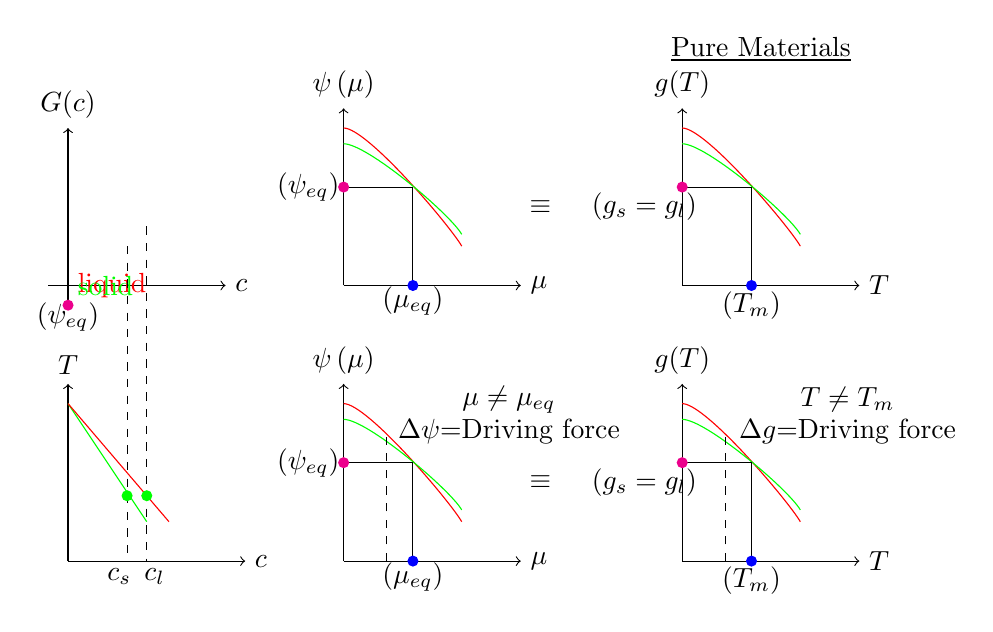
\begin{tikzpicture}[domain=0:1.75]
    %   \draw[very thin, color=gray] (0.0,1.7) grid (1.7,1.7);
    \begin{scope}
      \draw[->] (-0.25,0)--(2,0) node[right]{$c$};
      \draw[->] (0,-0.25)--(0,2) node[above]{$G(c)$};
      \draw[color=red] plot[id=x] function{((x-0.5)**2) + 0.5}
      node[right] {liquid};
      \draw[color=green] plot[id=x1] function{((x-0.25)**2) + 0.25}
      node[right] {solid};
      \draw[color=blue] plot[id=x2] function{3./4 + (x-1)};
      \fill[magenta] (0,-0.25) circle(2pt);
      \node at (0,-0.4){($\psi_{eq}$)};
    \end{scope}
    \begin{scope}[xshift=3.5cm]
    \draw[->] (0,0)--(2.25,0) node[right]{$\mu$};
    \draw[->] (0,0)--(0,2.25) node[above]{$\psi\left(\mu\right)$};
    \draw[red](0,2)..controls +(0:0.3) and +(120:0.3)..(1.5,0.5);
    \draw[green](0,1.8)..controls +(0:0.3) and +(120:0.3)..(1.5,0.65);
    \draw[] (0.88,1.25)--(0.88,0.0);
    \draw[] (0.0,1.25)--(0.88,1.25);
    \fill[blue] (0.88,0.0) circle(2pt);
    \node at (0.88,-0.2){($\mu_{eq}$)};
    \fill[magenta] (0.0,1.25) circle(2pt);
    \node at (-0.45,1.25){($\psi_{eq}$)};
    \node at (2.5,1){$\equiv$};
    \end{scope}
    \begin{scope}[xshift=7.8cm]
    \draw[->] (0,0)--(2.25,0) node[right]{$T$};
    \draw[->] (0,0)--(0,2.25) node[above]{$g(T)$};
    \draw[red](0,2)..controls +(0:0.3) and +(120:0.3)..(1.5,0.5);
    \draw[green](0,1.8)..controls +(0:0.3) and +(120:0.3)..(1.5,0.65);
    \draw[] (0.88,1.25)--(0.88,0.0);
    \draw[] (0.0,1.25)--(0.88,1.25);
    \fill[blue] (0.88,0.0) circle(2pt);
    \node at (0.88,-0.25){($T_m$)};
    \fill[magenta] (0.0,1.25) circle(2pt);
    \node at (-0.48,1.0){($g_s=g_l$)};
    \node at (1,3){\underline{Pure Materials}};
    \end{scope}
    \begin{scope}[yshift=-3.5cm]
    \draw[->] (0,0)--(2.25,0) node[right]{$c$};
    \draw[->] (0,0)--(0,2.25) node[above]{$T$};
    \draw[green] (0,2)--(1,0.5);
    \draw[red] (0,2)--(1.5/1.17,0.5);
    %  \draw[red] plot[id=x4] function{2.0-1.17*x};
    \draw[dashed] (3/4,3.5+1/2)--(3/4,0.0);
    \fill[green] (3/4,0.83) circle(2pt);
    \draw[dashed] (1,3/4+3.5)--(1,0.0);
    \node at (3/4-0.1,-0.2){$c_s$};
    \node at (1.1,-0.2){$c_l$};
    \fill[green] (1,0.83) circle(2pt);
    %  \draw[red](0,2)..controls +(0:0.3) and +(120:0.3)..(1.5,0.5);
    %  \draw[green](0,1.8)..controls +(0:0.3) and +(120:0.3)..(1.5,0.65);
    %  \draw[] (0.88,1.25)--(0.88,0.0);
    %  \draw[] (0.0,1.25)--(0.88,1.25);
    %  \fill[blue] (0.88,0.0) circle(2pt);
    %  \node at (0.88,-0.2){($\mu_{eq}$)};
    %  \fill[magenta] (0.0,1.25) circle(2pt);
    %  \node at (-0.45,1.25){($\psi_{eq}$)}; 
    \end{scope}
    \begin{scope}[xshift=3.5cm,yshift=-3.5cm]
    \draw[->] (0,0)--(2.25,0) node[right]{$\mu$};
    \draw[->] (0,0)--(0,2.25) node[above]{$\psi\left(\mu\right)$};
    \draw[red](0,2)..controls +(0:0.3) and +(120:0.3)..(1.5,0.5);
    \draw[green](0,1.8)..controls +(0:0.3) and +(120:0.3)..(1.5,0.65);
    \draw[] (0.88,1.25)--(0.88,0.0);
    \draw[] (0.0,1.25)--(0.88,1.25);
    \fill[blue] (0.88,0.0) circle(2pt);
    \node at (0.88,-0.2){($\mu_{eq}$)};
    \fill[magenta] (0.0,1.25) circle(2pt);
    \node at (-0.45,1.25){($\psi_{eq}$)};
    % \node at (2.5,2.95){\underline{Departure from equilibrium}};
    \draw[dashed](0.55,0.0)--(0.55,1.65);
    \node at (2.1,1.65){$\Delta \psi$=Driving force};
    \node at (2.1,2.05){$\mu\neq\mu_{eq}$};
    \node at (2.5,1){$\equiv$};
    \end{scope}

    \begin{scope}[xshift=7.8cm,yshift=-3.5cm]
    \draw[->] (0,0)--(2.25,0) node[right]{$T$};
    \draw[->] (0,0)--(0,2.25) node[above]{$g(T)$};
    \draw[red](0,2)..controls +(0:0.3) and +(120:0.3)..(1.5,0.5);
    \draw[green](0,1.8)..controls +(0:0.3) and +(120:0.3)..(1.5,0.65);
    \draw[] (0.88,1.25)--(0.88,0.0);
    \draw[] (0.0,1.25)--(0.88,1.25);
    \fill[blue] (0.88,0.0) circle(2pt);
    \node at (0.88,-0.25){($T_m$)};
    \fill[magenta] (0.0,1.25) circle(2pt);
    \node at (-0.48,1.0){($g_s=g_l$)};
    %  \node at (1,3){\underline{Pure Materials}};
    \node at (2.1,1.65){$\Delta g$=Driving force};
    \node at (2.1,2.05){$T\neq T_m$};
    \draw[dashed](0.55,0.0)--(0.55,1.65);
    \end{scope}
    \label{Drivingforcealloys}
    \end{tikzpicture}

  The formulation of a driving force for the case of say a binary alloy
  solidification can be derived analogically as for pure materials.
  Assuming conditions of local thermodynamic equilibrium(LTE) (which in the
  case of pure materials implies that the temperature of the solid and 
  liquid are equal at the interface), the driving force for phase
  transformation in alloys is the difference of the grand-potentials
  of the solid and the liquid phases (or the difference of the chemical
  potentials of any of the chemical entitities depending on whether we
  start from a Helmholtz free-energy density or a Gibbs-free energy 
  density in the functional). In the present description, we adopt a 
  Helmholtz free energy density which then results in the driving 
  force for solidification being described as $\Psi_l-\Psi_s$ in the same
  manner as $g_l-g_s$ for the case of pure materials solidification.
  The difference is, while the state-variable in the case of the pure
  material solidification is the temperature $T$, it becomes the 
  diffusion-potential $\mu$ in the case of binary alloy solidification.
  This analogy can be well appreciated from the diagramm in Fig \ref{Drivingforcealloys}.
  At equilibrium, the common-tangent construction gives the equilibrium
  compositions of the solid and liquid, which can be read from the 
  equilibrium phase diagram. This same equilibrium can also be represented
  as the intersection of the grand-potential densitities $\Psi\left(\mu\right)$ 
  expressed as a function of the diffusion-potentials $\mu$, where $\Psi_s\left(\mu_{eq}\right)
  =\Psi_l\left(\mu_{eq}\right)$, in the same manner as $g_s(T_m)= g_l(T_m)$ for
  the case of pure materials. Away from equilibrium  $\mu\neq\mu_{eq}, \Psi_l\neq \Psi_s$,
  and we have a driving force for phase transition given by the difference of the 
  grand-potential densities.
  
  Therefore, using this above analogy we can write down the driving force
  for phase transition for alloys purely in terms of the diffusion potential 
  $\mu$ by performing a Taylor series expansion around equilibrium, until first order as follows, 
  
  \begin{align}
  \Psi_s\left(\mu\right) &= \Psi_s\left(\mu_{eq}\right) + \dfrac{\partial \Psi_s}{\partial \mu}\left(\mu-\mu_{eq}\right)\\
  \Psi_l\left(\mu\right) &= \Psi_l\left(\mu_{eq}\right) + \dfrac{\partial \Psi_l}{\partial \mu}\left(\mu-\mu_{eq}\right).
  \end{align}
  
  From the fig. \ref{Drivingforcealloys} it is clear that we can express the 
  grand-potential as $\Psi(\mu) = g(c(\mu)) -\mu c\left(\mu\right)$, which is the 
  essentially the \textit{Legendre transform} of $g$. Therefore, we can derive, 
  
  \begin{align}
   \dfrac{\partial \Psi}{\partial \mu} &= \dfrac{\partial g}{\partial c}\dfrac{\partial c}{\partial \mu} - \mu \dfrac{\partial c}{\partial \mu} -c\\
                                       &= -c,
  \end{align}
  
  where we have used $\dfrac{\partial g}{\partial c}=\mu$. Clearly, then we can write 
  the driving force for solidification $\Psi_l-\Psi_s$ as,
  
  \begin{align}
   \Psi_l-\Psi_s &= (c_s^{eq} - c_l^{eq})\left(\mu-\mu_{eq}\right),
  \end{align}
  
  where we have used $\Psi_l\left(\mu_{eq}\right) = \Psi_s{\mu_{eq}}$ and $\dfrac{\partial \Psi_l}{\partial \mu}_{\mu_{eq}} = -c_l^{eq}$
  and $\dfrac{\partial \Psi_s}{\partial \mu}_{\mu_{eq}} = -c_s^{eq}$. This relation can be 
  transmitted in the evolution equation for the phase-field variable $\eta$ as,
  
  \begin{align}
  \dfrac{\partial \eta}{\partial t} &= -M \left(\dfrac{\partial f_o}{\partial \eta} - 2\kappa\nabla^{2}\eta\right)  
					-M\underbrace{(c_l^{eq} - c_s^{eq})\left(\mu-\mu_{eq}\right)\dfrac{\partial h\left(\eta\right)}{\partial \eta}}_{driving force}.
  \end{align}

  The time-update of the coupled variable $\mu$ can be achieved in the same manner 
  as we derived the evolution equation for the temperature from the conservation of
  the internal energy. The local composition writes as, 
  
  \begin{align}
   c = c_s h\left(\eta\right) + c_l (1 - h\left(\eta\right)), 
  \end{align}
  
  analogically as the internally energy before. More rigourously the above relation derives from the 
  interpolation of the grand-potential densities $\Psi\left(\mu\right) = 
  \Psi_s\left(\mu\right) h\left(\eta\right) + \Psi_l\left(\mu\right) (1 - h\left(\eta\right))$,
  and taking the derivative with respect to the diffusion potential lets us to the relation, 
  $\dfrac{\partial \Psi}{\partial \mu} = \dfrac{\partial \Psi_s}{\partial \mu} h\left(\eta\right) 
  + \dfrac{\partial \Psi_l}{\partial \mu} (1-h\left(\eta\right))$.
 
 Substituting the above relation between the compsition and the diffusion-potential
 into the mass-conservation equation we have, 
 
 \begin{align}
  \dfrac{\partial c}{\partial t} &= \nabla \cdot \left(M\nabla\mu\right)\\
 \left(\dfrac{\partial c_s}{\partial \mu}h\left(\eta\right) + \dfrac{\partial c_l}{\partial \mu}(1-h\left(\eta\right))\right)
 \dfrac{\partial \mu}{\partial t} &= \nabla \cdot \left(M\nabla\mu\right) 
 - \left(c_s\left(\mu\right) - c_l \left(\mu\right)\right)\dfrac{\partial h\left(\eta\right)}{\partial t}.
 \label{Mass-conservation-alloys}
 \end{align}
 
 Clearly, we can can compare the evolution equations obtained in 
 Eqn. \ref{energy-conservation-pure} and Eqns. \ref{Mass-conservation-alloys}.
 The first term on the right-hand side of both equations represent the
 diffusive fluxes, while the second-term on R.H.S of both equations represent
 the source-terms from phase transformation. While in the case of pure 
 material solidification this represents the latent heat of phase transformation, 
 for the case of isothermal alloy solidification, it is the amount of mass
 -transfer occurring as a result of solute re-distribution during phase transformation.
 Thus, we are able to derive the evolution equations for phase transformation of pure
 materials and alloys with a similar starting point of first deriving the driving 
 forces in terms of the relevant state variables and then coupling it with the 
 appropriate conservation equations.















\end{document}
